\documentclass[border=3pt,tikz]{standalone}
% Shared look for every TikZ figure in these notes.
% Included by each standalone figure file; also keeps the figures consistent
% with the colours used in the PDF and on the website.

\usepackage{tikz}
\usepackage{pgfplots}
\pgfplotsset{compat=1.18}
\usetikzlibrary{arrows.meta, decorations.markings, decorations.pathmorphing,
                patterns, calc, positioning}
\usepackage{amsmath}

% Series colours are the three validated categorical slots also used by the
% interactive widgets, so a path drawn in the printed notes and the same path on
% the website are the same colour. They clear the colour-vision-deficiency and
% contrast checks as a set; every path is direct-labelled as well, so colour is
% never the only thing carrying identity.
\definecolor{duPurple}{HTML}{68246D}
\definecolor{duBlue}{HTML}{2A78D6}
\definecolor{duRed}{HTML}{EB6834}
\definecolor{duGreen}{HTML}{1BAF7A}
\definecolor{duGrey}{HTML}{4D4D4D}

\tikzset{
  % heavier default lines and arrow tips, so diagrams stay clear when zoomed
  every picture/.append style = {line width=0.7pt, >={Stealth[length=3mm]}},
  axisline/.style   = {-{Stealth[length=3.4mm]}, line width=1.0pt, black},
  path1/.style      = {duBlue,   line width=1.6pt},
  path2/.style      = {duRed,    line width=1.6pt},
  path3/.style      = {duGreen,  line width=1.6pt},
  statedot/.style   = {circle, fill=black, inner sep=1.8pt},
  arrowhead/.style  = {decoration={markings,
                        mark=at position #1 with {\arrow{Stealth[length=3.4mm]}}},
                       postaction={decorate}},
  lbl/.style        = {font=\normalsize},
  slbl/.style       = {font=\small, duGrey},
  workfill/.style   = {duPurple, opacity=0.16},
}

% larger labels in plots as well
\pgfplotsset{every axis/.append style={label style={font=\normalsize}, tick label style={font=\small}, line width=0.9pt}}

% P6.6 solution sketch: CO2 in a cylinder/piston (the system) loses heat Q to
% the 20 C surroundings; the external force on the piston is proportional to V^3.
\begin{document}
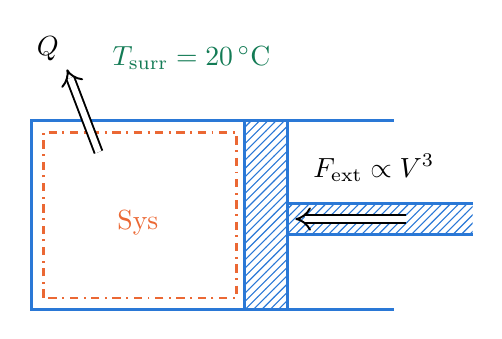
\begin{tikzpicture}[x=1cm,y=1cm,
    dbl/.style={double, double distance=2.2pt, line width=0.7pt,
                -{Implies[length=2.6mm]}, black}]
  % cylinder: closed on the left, open on the right
  \draw[duBlue, line width=1.1pt] (4.6,2.4) -- (0,2.4) -- (0,0) -- (4.6,0);
  % piston and rod (hatched)
  \fill[pattern=north east lines, pattern color=duBlue] (2.7,0) rectangle (3.25,2.4);
  \draw[duBlue, line width=1.1pt] (2.7,0) -- (2.7,2.4) (3.25,0) -- (3.25,2.4);
  \fill[pattern=north east lines, pattern color=duBlue] (3.25,0.95) rectangle (5.6,1.35);
  \draw[duBlue, line width=1.1pt] (3.25,1.35) -- (5.6,1.35) (3.25,0.95) -- (5.6,0.95);
  % system boundary, just inside the gas
  \draw[duRed, dash dot, line width=0.9pt] (0.15,0.15) rectangle (2.6,2.25);
  \node[lbl, duRed] at (1.35,1.1) {Sys};
  % heat out to the surroundings
  \draw[dbl] (0.85,2.0) -- (0.45,3.05) node[above left=-1pt, lbl] {$Q$};
  \node[lbl, duGreen!70!black, anchor=west] at (0.9,3.2) {$T_\text{surr} = 20\,^\circ$C};
  % external force on the piston
  \draw[dbl] (4.75,1.15) -- (3.35,1.15);
  \node[lbl, anchor=west] at (3.45,1.8) {$F_\text{ext} \propto V^{3}$};
\end{tikzpicture}
\end{document}
